%!TEX root = ../report.tex
\chapter{Requirements}
\label{ch:requirements}
This chapter will describe the vision and use it to derive stakeholders to be able to properly write use cases and stories. These will be used to extract functional, commercial, technical and evolution requirements. Afterwards, a risk assessment will take place, to ensure that the project is not at great risk.
%!TEX root = ../report.tex
\section{Architectural vision}

%!TEX root = ../report.tex
\section{Stakeholders and their concerns}

% wonder where do these factors come from

%kind of QA's (accourding to "Software Requirements" 3rd edition, Karll Wiegers and Joy Beatty)
%from page 263:

This section defines all stakeholders of our system and describe the concerns of the stakeholders. A stakeholder might be a person, group of persons, or organization that are involved in our system. There are eight stakeholders, ranged from first parties to third parties stakeholders. We use several quality standards from "Software Requirements" book by Microsoft \cite{wiegers2013software}. Those quality standards are described in \autoref{table:qa_standard}.

\begin{table}[!htbp] \centering
    \caption{Quality attributes of Software Architecture from "Software Requirements" Book \cite{wiegers2013software}.}
    \label{table:qa_standard}
    \begin{tabular}{L{\tw{0.2}} L{\tw{0.4}}}
    \toprule
    \textbf{Quality Attributes} & \textbf{Brief description} \\ \midrule
    Availability & The extent to which the system's services are available when and where they are needed\\
    Interoperability & How easily the system can interconnect and exchange data with other systems or components\\
    Performance & How quickly and predictable the system responds to user inputs or other events\\
    Reliability & How long the system runs before experiencing a failure \\
    Security & How well the system protects against unauthorized access to the application and its data\\
    Usability & How easy it is for people to learn, remember, and use the system\\
    \bottomrule
    \end{tabular}
\end{table}

There are six quality attributes, as can be seen in \autoref{table:qa_standard}, for measuring stakeholders' concern regarding our system. Furthermore, we also add profitability as another quality standard to improve measuring stakeholders' concern. Detailed description of stakeholders and their concerns are explained below.

% %from page 209 (Software Requirements book from microsoft):
% \todo{quote book, and ISO}
% Book and (ISO/IEC/IEEE 2011):\\
% \begin{tabular}{|L{\tw{0.2}}|L{\tw{0.4}}|}
% \toprule
% \textbf{Keyword} & \textbf{Priority} \\
% Shall & Required \\
% Should & Desired \\
% May & Optional \\
% \bottomrule
% \end{tabular}

\begin{description}
\item[Product owner] is concerned about the reliability and profitability of the system. The product owner funds the whole project and is highly concerned about the profitability. Thus, to gain big market share and extract large profit from this product, the product owner has to make this product reliable.
 
\item[Developers] are concerned about interoperability, performance and security. We, the architect team of RugSAG3 company, are also part of this. This stakeholder is responsible for the development of the systems until it is ready for production. Including architecting, designing, analyzing, testing and implementing this SFM System.

\item[Third party developers] are concerned about interoperability, availability, usability and reliability. Third party developers are important for our system since they need to provide an application that will give the users guidance in case of a flood.

\item[Competitors] are concerned about reliability and profitability. Competitors give negative effect on the system because competitors will be aiming on the same customer target. On the other hand, competitors are also triggering us to make a really good system in order to be able to compete with them and to save more lives. Thus, competitors must also be kept in consideration.

\item[Government] is concerned about availability and reliability. The government will be the main customer of this product, specifically, The Dutch Ministry of Infrastructure and the Environment. The government will be part of mitigation when the flood is imminent. This system will help the government by notifying them when it detects a flood and supplying them with relevant information about the flood.

\item[Citizens] are also concerned about availability and reliability, but also usability, since they can subscribe to warning by SMS. The Dutch residents are indirect user of this systems. Furthermore, they want this system to always be available and run correctly and notify them with reliable information.
% Guntur: I do not know the exact position of insurance companies in our stakeholders. Can anybody explain about this? Or should we just remove this stakeholder?

\item[Insurance companies] are concerned mostly about performance, reliability and availability. The damages caused by flood sometimes are also covered by the insurance companies. Thus, the insurance companies will also be part of the stakeholders and they will make sure that their business is running well.

\item[Local companies] are concerned about availability and reliability. Local companies will also be affected by the flood, since they have a lot of resources which are in danger. Local companies want to know whether or not this system is reliable so that they can arrange a proper action set when the flood comes to save their assets.

\item[Safety region] is responsible for the emergency services and is concerned about interoperability, performance, availability, reliability and usability. Emergency services are important when any accident happens, including flood. They will be really concerned about the thing that makes this system reliable, and inter-operable to their current system.
\end{description}

\autoref{table:stakeholder_concern} illustrates the stakeholder concern matrix. In our approach every stakeholders are equally the same. Thus, each stakeholder receives 100 points in total that has to be distributed among all the concerns.

\begin{table}[!htbp] \centering
	\caption{Matrix of stakeholders concern.}
	\label{table:stakeholder_concern}
    \begin{tabular}{@{} cl*{11}c @{}}
        &  & \multicolumn{7}{c}{\textbf{Concerns}} \\[2ex]
        & \textbf{Stakeholder} & \rot{Weight} & \rot{Availability} & \rot{Interoperability} & \rot{Performance} 
        & \rot{Reliability} & \rot{Security} & \rot{Usability} & \rot{Profitability}\\
        \cmidrule[1pt]{2-10}		
                     %   	   weight ava inte perf reli sec  usa  prof
        & Product owner			& 1	&    &    &    & 60 &    &    & 40 \\
        & Developers			& 1	& 	 & 40 & 30 & 	& 30 &    &    \\
        & Competitors 			& 1	&    &    &    & 40 & 	 &    & 60 \\
        & Government 			& 2	& 60 & 	  &    & 40 &    &    &    \\
        & Citizens				& 2	& 40 &    &    & 40 &    & 20 &    \\
        & Insurance companies	& 1	& 35 &    & 15 & 50 &    &    &    \\
        & Local companies		& 1	& 60 &    &    & 40 &    & 	  &    \\
        & Safety region			& 3	& 20 & 15 & 20 & 30 &    & 15 &    \\
        \cmidrule{2-10}
        & Total                	&	& 355& 85 & 105& 440& 30 & 85 & 100\\
        \cmidrule{2-10}
    \end{tabular}
\end{table}

As can be seen from \autoref{table:stakeholder_concern}, the most important concern of our system is the reliability, following availability as the second most important concern. This is also identical with our significant key driver.


% Key drivers
% high level requirements

%!TEX root = ../report.tex

%Citizen subscribes to service
%Sensor data is retrieved FR-1, FR-3, FR-5
%Weather data is retrieved FR-7
%Predict floud probability FR-8
%Get geo data FR-9
%The system should predict water levels FR-11, FR-12
%Monitor people should have access to a control panel FR-21

\clearpage


\section{Stories and use-cases}
This section will give an overview of the different use-cases. Figure \ref{fig:usecase-diagram} displays the use-case diagram. This provides an overview of the use-cases with their actors. In the subsections below, the architectural important use-cases are explained in more detail.

\begin{figure}[H]
	\centering
	\includegraphics[scale=0.35]{images/usecaseDiagramNew.png}
	\caption{Use-case diagram}
	\label{fig:usecase-diagram}
\end{figure}


%slides say:
%	Name & \\
%	Number & \\
%	Primary actor &  \\
%	Scope &  \\
%	Level &  \\
%	Extensions &  \\
%	Sub-variations & \\


\subsection{Receive sensor data}
\pgfplotstabletypeset[%
	UCTable
]{%
	value & description \\
	Number & \req{uc}\\
	Description & The system receives data from the different sensors deployed \\
	Stakeholders and interests & 
	\textbf{Developers}: Developers need to work with the sensor data \\
	Primary actor & System\\
	Scope & Monitoring part of the system \\
	Level & Sub process\\
	Precondition & The sensor is connected to a processing unit \\
	Main success scenario & \compactList{enumerate}{%
		\item The sensor does a measurement every 10 seconds
		\item The sensor sends the data to the central server every minute
		\item The central server normalizes the received data
		\item The central server stores the normalized data to the database
		\item The database stores the data
		}\\
	Postcondition & The database received and stored the sensor data \\
	Alternatives & \compactList{itemize}{%
		\item[2a.] 
		\begin{enumerate}
			\item The data cannot be sent
			\item Data will be lost
			\item The use-case ends 
		\end{enumerate}
		} \\
	Related requirements & \ref{fr:receive-waterlevel}, \ref{fr:receive-pressure}, \ref{fr:store-sensordata}, \ref{fr:retrieve-sensordata}\\
}

\clearpage
\subsection{Receive weather/GEO data}
\pgfplotstabletypeset[%
	UCTable
]{%
	value & description \\
	Number & \req{uc}\\
	Description & The system receives data from the weather forecast service \\
	Stakeholders and interests & 
	\textbf{Developers}: Developers would like to have a simple to use API \\
	Primary actor & System\\
	Scope & Monitoring part of the system \\
	Level & Sub process\\
	Precondition & The system needs external weather data to predict floods \\
	Main success scenario & \compactList{enumerate}{%
		\item The processing unit determines it needs forecast weather data%
		\item A call is made to the weather forecast service%
		\item The weather forecast service returns the requested data
		}\\
	Postcondition & The system received the forecast data \\
	Alternatives & \compactList{itemize}{%
		\item[3a.] 
		\begin{enumerate}
			\item The data cannot be returned.
			\item Repeat this process with another weather forecast service.
			\item If none are available, proceed monitoring without weather forecast data.
			\item After 5 minutes try to reconnect.
		\end{enumerate}
		}\\
	Related requirements & \ref{fr:receive-weather}\\
}

\clearpage
\subsection{Subscribing to SMS Service}
\pgfplotstabletypeset[%
	UCTable
]{%
	value & description \\
	Number & \req{uc}\\
	Description & Citizens can subscribe to the SMS service, so when a flood happens they will get a direct text message\\	
	Stakeholders and interests & 
	\textbf{Citizens}: Citizens want to be warned as soon as possible.
	\\
	Primary actor & Citizen\\
	Scope & Warning part of the system \\
	Level & User goal \\
	Precondition & Citizen has a mobile phone and is not subscribed to the SMS service \\
	Main success scenario & \compactList{enumerate}{
		\item Citizen sends a text message to our SMS service
		\item The SMS service receives the text message
		\item The SMS service sends the phone number to the SFM system
		\item The SFM system stores the phone number in the database
		\item A text message is sent back to the citizen with confirmation by the SMS service
		}\\
	Postcondition & Citizen is subscribed to the SMS service \\
	Alternatives & \compactList{itemize}{%
		\item[2a.] The text message is not received \\
		The use-case ends
		}\\
	Related requirements & \ref{fr:citizens-subscribe} \\
}

\clearpage
\subsection{Determining flood probability}
\pgfplotstabletypeset[%
	UCTable
]{%
	value & description \\
	Number & \req{uc}\\
	Description & The central processing unit calculates the probability of a flood \\
	Stakeholders and interests & \compactList{itemize}{%
		\item \textbf{Safety region}: The safety region wants to know when a flood warning is triggered
		\item \textbf{Government}: The government would also like to know when a flood warning is triggered
		}\\
	Primary actor & System\\
	Scope & Monitoring and warning part of the system\\
	Level & Sub process\\
	Precondition & The sensor data is available \\
	Main success scenario & \compactList{enumerate}{%
		\item The central processing unit gets the latest sensor data from the database
		\item The central processing unit gets the latest weather forecast data
		\item The central processing unit calculates the probability of a flood
		\item The central processing unit stores the probability value in the database
		\item The central processing unit determines that a flood is imminent based on the probability value
		\item A warning is send to the emergency services (they will warn the government)
		\item A warning is send to the citizens
		}\\
	Postcondition & The flood probability is calculated and stored. If the probability exceeds a certain threshold, a warning is sent to the authorities and citizens \\
	Alternatives & \compactList{itemize}{
		\item[5a.] The probability is not above the threshold \\
		The use-case ends
		}\\
	Related requirements & \ref{fr:detect-flood} \\
}

\clearpage
\subsection{Warn citizens in case of an imminent flood}
\pgfplotstabletypeset[%
	UCTable
]{%
	value & description \\
	Number & \req{uc}\\
	Description & Citizens who are subscribed to the SMS service will be warned through text messages in case of an imminent flood\\	
	Stakeholders and interests & \compactList{itemize}{
		\item \textbf{Citizens}: When they are subscribed, they want to be warned in case of an imminent flood
		}\\
	Primary actor & Citizen\\
	Scope & Warning part of the system \\
	Level & User goal \\
	Precondition & There is an imminent flood and the citizen is subscribed to the SMS service\\
	Main success scenario & \compactList{enumerate}{%
		\item The flood monitoring \& detection unit sends a warning about an imminent flood to the warning unit
		\item The warning unit queries the database for a list of phone numbers of subscribed citizens in the area
		\item The monitoring unit sends the collected phone numbers to the SMS service
		\item The SMS service sends a warning to all the collected phone numbers
		}\\
	Postcondition & The citizens who are subscribed received a warning\\
	Alternatives & \compactList{itemize}{%
		\item[3a.] 
		\begin{enumerate}
			\item A message cannot be sent to the citizen
			\item Wait a minute and resend
			\item The use-case ends
		\end{enumerate}
		}\\
	Related requirements & \ref{fr:warn-citizens} \\
}

\clearpage
\subsection{Warn safety region in case of an imminent flood}
\pgfplotstabletypeset[%
	UCTable
]{%
	value & description \\
	Number & \req{uc}\\
	Description & The safety region needs to receive a warning about an imminent flood\\
	Stakeholders and interests & \compactList{itemize}{%
		\item \textbf{Government}: The government wants to warn the citizens in case of a flood
		\item \textbf{Safety regions}: The emergency services want to help the citizens in case of a flood
		}\\
	Primary actor & Safety region \\
	Scope & Warning part of the system \\
	Level & User goal \\
	Precondition & There is an imminent flood\\
	Main success scenario & \compactList{enumerate}{
		\item The processing unit determines what area will be under water in case of a flood
		\item The processing unit determines how many people will be affected by the imminent flood
		\item The processing unit predicts how the flood will develop in the following period 
		\item The processing unit will create a map based on the current state and predictions
		\item The processing unit sends the map to the government and emergency services
		}\\
	Postcondition & A map with current and predicted data is sent to the government and emergency authorities \\
	Related requirements & \ref{fr:compute-area}, \ref{fr:analyze-waterlevel}, \ref{fr:estimate-waterlevel}, \ref{fr:compute-nrcivilians}, \ref{fr:warn-safetyregion} \\
}

\clearpage
\subsection{Third party accessing data through the systems API}
\pgfplotstabletypeset[%
	UCTable
]{%
	value & description \\
	Number & \req{uc}\\
	Description & Third parties can use the API exposed by the flood monitoring system in third party applications (providing guidance to citizens) \\
	Stakeholders and interests & \compactList{itemize}{%
		\item \textbf{Third parties}: Third parties want to access the data of the flood monitoring system to use in their applications
		\item \textbf{Citizens}: Citizens want to receive guidance in case of a flood.
		}\\
	Primary actor & Third party \\
	Scope & The API part of the system \\
	Level & User goal \\
	Precondition & The third party has access to the flood monitoring systems API \\
	Main success scenario & \compactList{enumerate}{
		\item The third party application connects to the API
		\item The third party application sends a request for certain data to the API
		\item The system retrieves the requested data from the database
		\item The system sends the retrieved data to the third party application
		}\\
	Postcondition & The third party application has received the requested data \\
	Related requirements & \ref{fr:expose-api} \\
}

\clearpage
\subsection{Detecting a faulty sensor}
\pgfplotstabletypeset[%
	UCTable
]{%
	value & description \\
	Number & \req{uc}\\
	Description & The system is able to detect when a sensor is not functioning properly \\
	Stakeholders and interests & \compactList{itemize}{%
		\item \textbf{Product owner}: The product owner wants the system to be reliable and errors/broken sensors to be fixed
		}\\
	Primary actor & The system \\
	Scope & The monitoring part of the system \\
	Level & Sub process \\
	Precondition & The sensor is not functioning properly \\
	Main success scenario & \compactList{enumerate}{
		\item The system receives the sensor data
		\item The system compares the sensor data with other information, including data of nearby sensors and previous data of this sensor 
		\item The system detects that this reading is abnormal, but determines it cannot be caused by an (imminent) flood
		\item The system ignores further readings from this sensor and reports the faulty sensor in the control panel
		}\\
	Postcondition & The faulty sensor is not used in future measurements and is reported in the control panel \\
	Alternatives & \compactList{itemize}{%
		\item[3a.] 
		\begin{enumerate}
			\item The system cannot determine the abnormal reading is not caused by a flood
			\item The system keeps using this sensors data, until it can determine that the readings are not caused by a flood, or it determines that it is caused by a flood (in which case it will issue warnings, see \hyperref[uc:4]{UC-4})
		\end{enumerate}
		}\\
	Related requirements & \ref{fr:detect-faultysensor}, \ref{fr:report-faultysensors}, \ref{fr:controlpanel-warnings}, \ref{fr:controlpanel-errors}, \ref{fr:controlpanel-sensors}
	\\
}

\clearpage
\subsection{Maintenance employee checks system state}
\pgfplotstabletypeset[%
	UCTable
]{%
	value & description \\
	Number & \req{uc}\\
	Description & A maintainer of the system regularly checks the state of the system in the control panel to see if there are errors or sensors that need maintenance. \\
	Stakeholders and interests & \compactList{itemize}{%
		\item \textbf{Product owner}: The product owner wants the system to be reliable and errors/broken sensors to be fixed
		}\\
	Primary actor & Maintainer \\
	Scope & The maintenance part of the system \\
	Level & User goal \\
	Precondition &  \\
	Main success scenario & \compactList{enumerate}{
		\item The maintainer uses his login credentials to get access to the control panel
		\item The maintainer navigates to the errors/warning page
		\item The maintainer checks on this page if there are problems with the system (errors/warning)
		\item The maintainer takes necessary action to resolve any issues
		}\\
	Postcondition & The maintainer is aware of reported problems with the system \\
	Related requirements & \ref{fr:controlpanel}, \ref{fr:report-faultysensors}, \ref{fr:controlpanel-warnings}, \ref{fr:controlpanel-errors}, \ref{fr:controlpanel-sensors} \\
}



%!TEX root = ../report.tex
\section{Functional requirements}
\begin{longtable}{p{0.1\textwidth} p{0.1\textwidth} p{0.8\textwidth}}
    \textbf{Nr.} & \textbf{Prio}  & \textbf{Description} \\
    
    \hline \phantomsection \label{fr:1} FR-1 & 
    \phantomsection  \textbf{Must} &
    \phantomsection  The system is able to receive and process input from sensors with regards to the water level. This information will be used to determine if there is an imminent flood. \\
    
    \hline \phantomsection \label{fr:2} FR-2 & 
    \phantomsection  \textbf{Must} &
    \phantomsection  The system is able to receive and process input from sensors with regards to the pressure/consistency of the dykes. This information will be used to determine if there is an imminent flood. \\
    
    \hline \phantomsection \label{fr:3} FR-3 & 
    \phantomsection  \textbf{Must} &
    \phantomsection  The system retrieves weather forecasting data from weather forecasting services. The retrieved weather forecasting data consists of predictions about the precipitation and wind data. This data will be used by the system to help in determining when a flood becomes imminent.
     \\
     
    \hline \phantomsection \label{fr:4} FR-4 & 
    \phantomsection  \textbf{Must} &
    \phantomsection  The system is able to detect from the sensor data and weather forecast information when a flood is imminent. \\ % what are the criteria for an imminent flood??
    
    \hline \phantomsection \label{fr:5} FR-5 & 
    \phantomsection  \textbf{Must} &
    \phantomsection The system can compute (from geographic information) the area which will be affected by a flood. \\
    
    \hline \phantomsection \label{fr:6} FR-6 & 
    \phantomsection  \textbf{Must} &
    \phantomsection The system is able to collect information pertaining to the severity of the flood. The severity can be deducted from the expected water level, how fast the water level in the flood area will rise, and by the number of civilians living in the affected area (population density). \\
    
    \hline \phantomsection \label{fr:7} FR-7 & 
    \phantomsection  \textbf{Must} &
    \phantomsection The system provides emergency services with information about the flood. This includes the area affected by the flood and information needed to deduct the severity of the flood. \\
    
	\hline \phantomsection \label{fr:8} FR-8 & 
    \phantomsection  \textbf{Must} &
    \phantomsection  When a flood is imminent, the system should send a warning to the emergency services and to the authorities.\\
    % what info is in the warning
    % who is that: authorities?
    
    \hline \phantomsection \label{fr:9} FR-9 & 
    \phantomsection  \textbf{Must} &
    \phantomsection  The system is able to compute a safe route to a safe area where citizens can be evacuated to in case of an (imminent) flood. \\    

    \hline \phantomsection \label{fr:10} FR-10 & 
    \phantomsection  \textbf{Must} &
    \phantomsection  When a flood is imminent, the system should send a warning to citizens who are subscribed for such warnings. This warning will contain information about how to get to a safe area. \\
	
    \hline \phantomsection \label{fr:11} FR-11 & 
    \phantomsection  \textbf{Must} &
    \phantomsection  The system is able to predict the development of the water level. This information can be used to predict how fast a flood will develop. \\
	
    \hline \phantomsection \label{fr:12} FR-12 & 
    \phantomsection  \textbf{Must} &
    \phantomsection The system uses different sources to confirm imminent flood warnings, in order to limit false positives. \\% not very specific yet
	
    \hline \phantomsection \label{fr:13} FR-13 & 
    \phantomsection  \textbf{Must} &
    \phantomsection The system can detect a faulty sensor, either when the sensor raises an error or when the data from the sensor is inconsistent with other sensor data. \\
	
    \hline \phantomsection \label{fr:14} FR-14 & 
    \phantomsection  \textbf{Must} &
    \phantomsection The system can report faulty sensors, so these sensors can be repaired or replaced. \\ %how will it be reported and to whom?? \\
    
	\hline \phantomsection \label{fr:15} FR-15 & 
    \phantomsection  \textbf{Must} &
    \phantomsection In case of a flood, the system will provide emergency services with safe routes to incident locations. \\
    
    \hline \phantomsection \label{fr:16} FR-16 & 
    \phantomsection  \textbf{Must} &
    \phantomsection Citizens are able to subscribe to flood warning messages. \\
    % TODO: we need to decide how citizens will subscribe: web page, app??
    
    \hline \phantomsection \label{fr:17} FR-17 & 
    \phantomsection  \textbf{Must} &
    \phantomsection The system has access to geographic information, including road data and terrain height data. \\
    
    \hline \phantomsection \label{fr:18} FR-18 & 
    \phantomsection  \textbf{Must} &
    \phantomsection The system can determine the area affected by a flood, by using the location data of the sensors and geographic information. \\
    
    \hline \phantomsection \label{fr:19} FR-19 & 
    \phantomsection  \textbf{Must} &
    \phantomsection The system can determine the location of the citizen, after he/she is warned about a flood, in order to compute a safe route to a safe area. \\
    
    \hline \phantomsection \label{fr:20} FR-20 & 
    \phantomsection  \textbf{Must} &
    \phantomsection The system can determine the location of an emergency vehicle, so it is able to compute a safe route to incident locations. \\
    
    
	
    \hline \phantomsection \label{fr:21} FR-21 & 
    \phantomsection  Future &
    \phantomsection The system is able to detect extreme weather phenomena, like storms etc. \\
\end{longtable}

%!TEX root = ../report.tex
\section{Commercial non functional requirements}
 In this section commercial non functional requirements are presented.
 
\textbf{CNFR-1} The system is affordable.
The selling price of the system to the authorities is about *********** euros per city or municipality. This price is lower than 70\%\ of the competitors price. % How to calcuatenthe selling price , do we need to give it ?

%\textbf{CNFR-2} The maintenance costs are ********** euros.

\textbf{CNFR-2} The sensors have a good quality , the sensors companies have good ratings so we don't have replace the sensors often => less money spent on repairs. The guarantee of the sensors should be about three years.

IDEAS :
\textbf{CNFR-} A video explains how the system works to the end-users : authorities and emergency services.
\textbf{CNFR-} Advertissement ???

%!TEX root = ../report.tex
\section{Technical non-functional requirements}
In this section, the technical non-functional requirements important to this system are discussed.

\subsection{Resilience}
The system will have many connected sensors, which can have failures. The system should be able to recognize such failures timely and recover from them without the QoS or the functionality of the system being affected. 

The system should be able to continue functioning with the same QoS in a situation where up to 5\% of the sensors suffer from failures.  % WM: is 5% realistic?

\subsection{Interoperability}
The system has dependencies on third-party systems. For example, to make predictions about the development of waterlevel, the system will need to retrieve information from water forecasting services. 

Not only for input, but also for output, the system will need to interoperate with third-party systems. If the system has registered a risk of a flood, it should interact with systems of emergency services and other authorities to alert them and sent relevant information.
% TODO: how to measure? 

% ============================================================
% From Gerrit:
% The three main requirements:
% 1: Monitoring activities: the system should monitor activities and properties of
% rivers, waterways, dykes, such as the water level and pressure or the consistency
% of the dyke. Monitoring can be performed through different devices, e.g. analog
% and digital sensors, Unmanned Aerial Vehicles (UAVs) and Vehicular Ad-hoc
% Networks (VANETs) etc.
% 2: Warning: in case of an imminent flood, the system should issue warnings to the
% authorities and emergency services, but also directly to citizens who are
% subscribed for such messages (e.g. through SMS or mobile apps).
% 3: Guidance: the system should provide runtime information to guide its
% constituents or third parties, .e.g. the UAVs may provide information to
% VANETs embedded in vehicles crossing the area, thereby guiding vehicles
% driving towards a flood area to avoid certain routes. Meanwhile, the VANETs
% can also provide an alternative route to emergency services or citizens to avoid
% the flood area. 

% ToDo:
% Stakeholders
% Use-cases
% Make them smart
% Assign value (must/should/...
% ============================================================


 %%!TEX root = ../report.tex}
\section{Evolution requirements}
%\label{subsec:evolrequir}

%Typical change-cases with respect to the environement, the features and the technology of the system
%http://www.agilemodeling.com/artifacts/changeCase.htm
When establishing the project, architects of the system listed a certain number of requirements which describe the features of the system. However, due to environmental changes and changing stakeholder interests, for example, the requirements may evolve.

%\textbf{ER-1 : Changes in the display of the map } \\
%\textit { Evolution of \ref{fr:construct-map}}. Citizens who subscribed for flood warnings get a map with specific route information (according to their location) to a safe area through the API. \\

%\begin{longtable}{L{0.1\textwidth} L{0.12\textwidth} L{0.7\textwidth}}
	%\textbf{Nr.} & \textbf{Name}  & \textbf{Description} \\


\textbf{ER-1 : Adding of external input}\\
 Citizens can contribute to the guidance by giving extra information (for example if they identified a safe route near their location). This information can be checked by an operator (thanks to photograph by the UAVs for example). 
 
 Functionality can be added to the system in the future, that can take citizen feedback into account for the flood prediction.
 \\
 
\textbf{ER-2 : New sensors } The system is able to work with new sensors technologies, which are coming on the market over the years. \\

\textbf{ER-3 : Improved algorithms for detecting a flood} \\
New algorithms may become available, which have a better accuracy for the flood prediction described in \ref{fr:detect-flood}. The part of the system with the flood prediction algorithm has to be modular, so that it can be replaced with an improved algorithm, once such an algorithm becomes available.

	%\bottomrule
%\end{longtable}


%\textbf{ER-3 : New OS } \\
%The system is able to work with other operating systems than Linux, for example Windows and MacOS. %Portability

%\textbf{ER-3} The system is able to work on several mobile devices platforms : Android, iOs, Windows Phone. \\ IN CASE OF AN APP
% GK: Im all for dropping evolution requirements, as there are hardly any metrics to measure it, while it's also quite hard to already define what's going to happen to the project after development. Also; it's not in the example, so where does this even come from? Evolution could be handled in a seperate chapter, but that should be more about ideas, rather than about requirements.

%!TEX root = ../report.tex
\newpage
\section{Risk assessment}
\label{sec:risk-assesment}
The system is confronted by several risks which are determined and mitigated in this section.
Taking those risks into account allows to avoid them or at least reduce their impact. 
The risk management involves the identification of the risks, their probability and potential impact or consequences.

The tables below explain the meaning of the definition for probability and consequence.
\begin{figure}[H]
	\centering
	\begin{tabular}{|c|c|}
		\hline \textbf{Probability} & \textbf{Likelihood of occurrence} \\ 
		\hline High                 & 0.65 - 1.00                       \\ 
		\hline Medium               & 0.35 - 0.65                       \\ 
		\hline Low                  & 0.00 - 0.35                       \\ 
		\hline
	\end{tabular} 
	\label{table:risk-probability}
\end{figure}

\begin{figure}[H]
	\centering
	\begin{tabular}{|l|p{15.5cm}|}
		\hline \textbf{Severity} & \textbf{Explanation}                                                                                                                        \\ 
		\hline Severe            & A risk that can lead to loss of live or casualties.                                                                                         \\ 
		\hline Significant       & A risk that can lead to damages, can delay the project more than 3 months or causes one of the high-level requirements not to be fulfilled. \\ 
		\hline Moderate          & A risk that can lead to one of the high-level requirements not to be fulfilled to an acceptable level.                                      \\ 
		\hline Minor             & A risk that can lead to one of the high-level requirements not being fully fulfilled, but still fulfilled in an acceptable level.           \\
		\hline
	\end{tabular} 
	\label{table:risk-severity}
\end{figure}

%Risk impact assesment and Prioritization
% Probability of Occurrence ( In the appendice is the table to which show how to evaluate a risk and the severity of consequences 
%\textit{http://www.mitre.org/publications/systems-engineering-guide/acquisition-systems-engineering/risk-management/risk-impact-assessment-and-prioritization} \\ % COSTS
%Timeframe is classified in : Long , Medium , Short , Imminent \\
%Consequences are classified in : Low, Moderate , High , Severe


%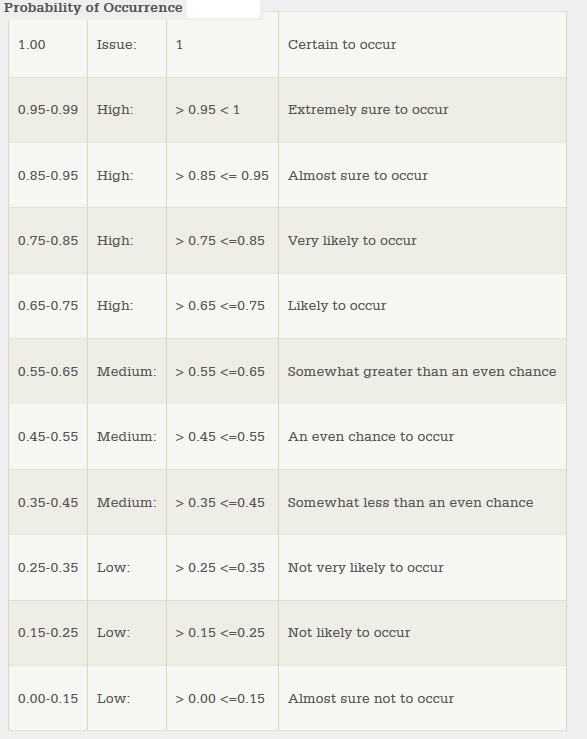
\includegraphics[scale=0.5]{3-requirements/Images/RISKSOCCURENCE.jpg} % maybe in the appendice ?
\subsection{Technical}

\risk{T}
{The system does not detect a flood}
{Low}
{Severe. There can be a loss of human lives and damages, loss of trust in the system by end-users.}
{Make sure the number of sensors is sufficient and that they are in good state (as low failure rate as possible, when necessary repair or replace them). Perform regular checks of the sensors. Make sure faults in sensors are reported. }
{Make changes in the algorithm for the flood detection, add more and new sensors which have good rates according to quality tests.}
{risk:flood-detect}

\risk{T}
{The system sends warnings of a non-existing flood (false positive)} % WHEN THERE IS A FLOOD YOU KNOW IT
{Low}
{Significant. People can become more negligent to future messages and unneeded social disturbance can be caused.}
{UAVs watching the area where the supposed flood is to confirm.}
{Send a message as soon as the mistake is detected to tell the population/emergency center it was a false alert. }
{risk:warning-nonexisting}

\risk{T}
{The system cannot send messages to the necessary people because the communication platform is also destroyed by the flood}
{Medium}
{Severe. If the warning is not send, the area might not be evacuated timely. Potential loss of human lives, casualties and damages to property. }
{}
{Send the warning to the safety board using a different medium.}
{risk:cantwarn}
	
\risk{T}
{The config panel is not checked often enough and broken sensors are not fixed}
{Low}
{Moderate. The accuracy and reliability of the system diminish if less sensors are available to the system.}
{Make sure there is a clear schedule for maintenance personnel to check the control panel.}
{Repair/replace all the sensors which were not repaired timely}
{risk:configpanel-notchecked}
	
%\risk{T}
%{The system sends incorrect information}
%{Low}
%{Severe. Loss of money and maybe lives.}
%{Operator checking the validity of the information sent by the system.
%	Good collaboration with the insurance companies.}
%{  }
% WM: Risk and severity depend highly on what kind of information is send incorrectly.

\risk{T}
{Hacker gets access to the system}
{Low}
{Severe. The hacker may sent incorrect information deliberately during the flood. This can cause unneeded evacuation, but in the case of a flood also loss of human lives. The system is not reliable anymore.}
{Change password and hash codes every three months. Hire specialists in the security field to audit the security system on a regular basis (penetration testing).}
{Update the security system / change it. Find a new algorithm for the creation of password and hash codes.}
{risk:hacker}

\risk{T}
{UAV cannot fly because of the weather}
{Medium}
{Moderate. If the UAV cannot fly, the system cannot use the data it would have collected for the flood probability computation.}
{Bad weather cannot be prevented. Use UAVs which can fly in suboptimal weather conditions.}
{If the UAV really cannot fly and the system is not sure about the flood probability, lower the threshold for warning safety region/citizens.}
{risk:uav-badweather}

\risk{T}
{Arduino becomes unavailable}
{Low}
{Minor. The Arduino has a limited number of attached sensors, so the consequences of a single Arduino failures are not too large.}
{Install the Arduino in such a way, that it is not exposed to external forces (like bad weather). This will decrease the odds of an Arduino failure.}
{The broken Arduino is reported in the control panel (several failing sensors) and should be replaced/repaired by maintenance personnel.}
{risk:arduino-broken}

\risk{T}
{SMS Service goes offline when there is a flood}
{Low}
{Moderate. The SMS Service is essential to warn citizens, which is a significant part of high-level requirement \ref{HL:2}.}
{Make sure the SMS Service which is used has good availability guarantees.}
{Use an alternative SMS Service or coordinate with the SMS Service provider to get the service back online.}
{risk:sms-service-online}



\subsection{Business}

\risk{B}
{Wrong estimation of the budget}
{Medium}
{Significant. The final product does not have the features expected.}
{The team needs an accountant or at least someone taking care of the follow-up of the money. Make sure there are regular evaluations to keep track of the money flow.}
{Remove some requirements or features of the product, or change the hardware components used.}
{risk:budget}

\risk{B}
{The money invested in the fabrication and achievement of the product/system is not covered by the sales (shortfall/deficit)}
{Medium}
{Moderate. Stopping the sale}
{The team needs an accountant or at least someone taking care of the follow-up of the money.}
{Adding more features to the product in order to make it more competitive in the market.}
{risk:shortfall}

\risk{B}
{Third-party developers do not build third-party applications using the systems API}
{Medium}
{Moderate. Without third-party applications, the citizens do not receive guidance in case of a flood}
{ Make sure the API exposes all features which are relevant to develop a third-party application for guidance. }
{ Promote the use of the API by third-party developers using, for example, a contest. }
{risk:3rdparty}

%\risk{B}
%{Competitors lowering their prices}
%{Medium}
%{Moderate. Loss of money.}
%{  }
%{  }
% WM: I think this one is too generic
	
\risk{B}
{Sensor becomes unavailable (is not sold anymore)}
{Medium}
{Moderate. Sensors will fail and need replacing over time, if new sensors are not available anymore, this becomes impossible.}
{ Choose a sensor that is not too old and is expected to be available for at least the next 5 years. }
{ Use a different sensor and modify the system so it can operate with this sensor. }
{risk:sensor-notsold}

%\textbf{ B-RISK4 The sensors company become bankrupt or at least stops its sales.} \\
%\textit{Probability of Occurence}: Low \\
%\textit{Consequences}: High.\\
%\textit{Prevention} Our system use sensors from different companies \\
%\textit{Decision}: Find another company selling sensors and make sure of its reliability. \\


\subsection{Schedule}
\risk{S}
{The project is not finished at the deadline}
{Low}
{Significant. Pressure for all the team members, loss of credibility regarding the customers, selling a product with less features than expected.}
{ SRA , Schedule Risk analysis : Estimation of the duration of the project by its manager ( with the use of probability and statistics ) . Meeting for the team members every week to keep track of the timing and take decisions according to the deadline. }
{ Postpone the deadline or remove some features when the deadline can't be postponed. }
{risk:schedule}
